\documentclass{article} % For LaTeX2e
\usepackage{nips13submit_e,times}
\usepackage{hyperref}
\usepackage{url}
\usepackage{amsmath}
\usepackage{graphicx}
\usepackage{float}
\usepackage{caption}
\usepackage{subcaption}
\floatplacement{figure}{H}
%\documentstyle[nips13submit_09,times,art10]{article} % For LaTeX 2.09


\title{Fast Support Vector Data Descriptions for Novelty Detection\\ Project Report\thanks{As a part of the course Kernel Methods for Pattern Analysis - CS6011 Jan - May 2015}}



\author{
Aravind Sankar \\
CS11B033 \\
Department of Computer Science\\
IIT Madras\\
\texttt{aravindsankar28@gmail.com} \\
\And
Adit Krishnan \\
CS11B063\\
Department of Computer Science\\
IIT Madras\\
\texttt{adit101293@gmail.com} \\
}

% The \author macro works with any number of authors. There are two commands
% used to separate the names and addresses of multiple authors: \And and \AND.
%
% Using \And between authors leaves it to \LaTeX{} to determine where to break
% the lines. Using \AND forces a linebreak at that point. So, if \LaTeX{}
% puts 3 of 4 authors names on the first line, and the last on the second
% line, try using \AND instead of \And before the third author name.

\newcommand{\fix}{\marginpar{FIX}}
\newcommand{\new}{\marginpar{NEW}}

\nipsfinalcopy % Uncomment for camera-ready version

\begin{document}


\maketitle

\begin{abstract}
The abstract paragraph should be indented 1/2~inch (3~picas) on both left and
right-hand margins. Use 10~point type, with a vertical spacing of 11~points.
The word \textbf{Abstract} must be centered, bold, and in point size 12. Two
line spaces precede the abstract. The abstract must be limited to one
paragraph.
\end{abstract}




\section{Brief Summary}
\subsection{Introduction}

In this paper, the authors address the common well-studied problem of Novelty Detection. In this task, we have a 2-class problem denoted by the normal and abnormal class points, where the number of points of abnormal class is lesser than that of the normal class. We note that this problem is different from the traditional classification problem in that only points of the normal class are used for the purpose of training, essentially a One-Class classification problem.  \\[10pt]

The Support Vector Data Description (SVDD)[1]  is an important and popular technique which has been used to solve the problem of Novelty Detection. In short, SVDD tries to construct a soft minimal hypersphere enclosing the points of the target class (normal) in the kernel feature space ($\phi$). This hypersphere boundary in the kernel feature space is used for prediction to identify the outlier points (novel data). SVDD like any other SVM, has a prediction time complexity linear in the number of support vectors ($N_s$) because $N_s$ evaluations of the kernel function is required for predicting the label of an unseen data point. \\[10pt]

The authors attempt to address this key issue in this paper by proposing Fast SVDD (F-SVDD) [2] which replaces the kernel expansion (of $N_s$ terms) in the decision function with just 1 term. This is achieved by first looking for a vector (called agent of the center) in the $\phi$-space whose preimage $\hat{x}$ exists in the $x$-space. Then, they express the sphere center $a_{\phi}$ as a scalar multiple of this vector in the $\phi$-space. Now, it can be seen the decision function involves only one kernel function between $\hat{x}$ and any unseen data point $x$. This means that the prediction time complexity is constant, irrespective of the size of the training dataset. The authors also propose an efficient method for solving the preimage problem, which is non-iterative and faster than the existing techniques. The way they solve these problems will be explained in the further sections.


\subsection{SVDD and some properties}
In this section, we introduce the SVDD problem definition for the purpose of notation. \\[10pt]

\textbf{Primal problem :}
\begin{equation}
\begin{split}
\text{min} \; R^2 + C \sum\limits_{i=1}^N \xi_i \\
\text{subject to}\\
||\phi(x_i) - a_{\phi}||^2  \leq R^2 + \xi_i \\
\xi_i \geq 0 \; \forall i = 1,...N
\end{split}
\end{equation}

\textbf{Dual problem:}

\begin{equation}
\begin{split}
\text{max}\; 1 - \sum\limits_{i=1}^N \sum\limits_{j=1}^N \alpha_i \alpha_j K(x_i,x_j) \\
\text{subject to}  \\
\sum\limits_{i = 1}^N \alpha_i  = 1  \\
0 \leq \alpha_i \leq C \;\; \forall  i = 1,...,N.  
\end{split}
\end{equation}


Here, the discriminant function $g(x)$ is given by :

\[ g(x) = ||\phi(x_i) - a_{\phi}||^2 - R^2 = c - 2 \sum\limits_{i=1}^{N_s}\alpha_i K(x,x_i) \]
where $c$ is a constant. \\[10pt]

The sphere center $a_\phi$ is given by :

\[ a_\phi  = \sum\limits_{i=1}^{N} \alpha_i \phi(x_i) = \sum\limits_{i=1}^{N_s} \alpha_i \phi(x_i)\]

We also compute $||a_\phi||$ as it will be used later, 
\begin{equation} \label{norm}
||a_\phi||^2 = ||\sum\limits_{i=1}^{N_s} \alpha_i \phi(x_i) ||^2  = \alpha^T K \alpha
\end{equation}

where $K$ is the kernel gram matrix. \\[10pt]


Let's denote the soft minimal hypersphere (constructed by SVDD over the training points) as $B_S$. We assume the use of a gaussian kernel function (can  be extended for any normalized kernel also)so that $K(x,x) = 1$. So, all points $\phi(x)$ lie on a unit hypersphere (centered at origin $O_\phi$) in the kernel feature space, denoted by $B_\phi$. This leads to interesting geometrical properties in the kernel feature space. One main property is mentioned below : \\[10pt]

\textbf{Property :} The center $a_\phi$ of the SVDD hypersphere $B_S$ must lie inside the unit hypersphere $B_{\phi}$. \\[10pt]


This property shows that the exact preimage of $a_\phi$ in the x-space does not exist. This means that, either only an approximate preimage can be found, or a different way needs to be found. F-SVDD does this by identifying the \textit{agent} of the center whose pre-image exists in the x-space. The following sections explain the process of finding the agent and it's preimage.


\subsection{Fast SVDD}
The main objective of F-SVDD is to improve classification speed by reducing the number of computations at prediction time. By the above property, the preimage of the center $a_\phi$ does not exist. This algorithm  
first defines the agent of the center.

\subsubsection{Agent of the center}

Let's denote the agent of the center $\Psi_a$ (in the kernel feature space). We want $\Psi_a$ to have a pre-image $\hat{x}$ in the x-space.  This directly implies that $\Psi_a$ should lie on the unit hypersphere  $B_{\phi}$ centered at Origin in the kernel feature space. This gives us  

\begin{equation}\label{norm1}
||\psi_a|| = 1 
\end{equation}

$\Psi_a$ is identified as the point closest to $a_\phi$ that lies on $B_{\phi}$. This point is obtained by  extending $a_\phi$ to intersect $B_\phi$. obviously is in the direction of $a_\phi$.
Thus, we can express $\Psi_a$ as :

\begin{equation}
\begin{split}
\Psi_a &= \gamma a_\phi \\\\
&\text{where } \gamma  \text{ is a scalar.} \\ \\
||\Psi_a|| &= \gamma ||a_\phi||  \\
\gamma &= \frac{1}{||a_\phi||}  \text{  (Using  \ref{norm1})} \\ 
\gamma &= \frac{1}{\sqrt{\alpha^T K \alpha}} \text{  (Using  \ref{norm})} 
\end{split}
\end{equation}


We also note that $\gamma >1$ as $||a_\phi|| < 1$.

This shows us that if we are able to obtain the preimage of the agent, the computation of our discriminant function reduces to just 1 term, which involves just $\hat{x}$. In the next section, we describe how the pre-image is computed for the agent.



\subsubsection{Preimage of the agent :}

Formally, we define the preimage problem as, given a feature vector $\psi$ in the kernel feature space, find $\hat{x} \in \mathbf{R}^d $ (x-space) such that $\psi = \phi(x)$.
The preimage $\hat{x}$ is found by solving the problem :

\[ \hat{x} = \min_{\hat{x}} ||\Psi_a - \phi(\hat{x}) ||^2   \]

It can shown that solving this problem is equivalent to finding the approximate preimage of $a_\phi$, i.e.

\[ \min \rho = ||a_\phi - \phi(\hat{x}) ||^2 \]


To minimize $\rho$, we set the derivative of the objective function ($\rho$) to 0 and we obtain : 

\[ \hat{x} = \frac{\sum\limits_{i=1}^N \alpha_i K(\hat{x},x_i)x_i}{\sum\limits_{i=1}^N K(\hat{x},x_i)} \]

We see that $\hat{x}$ appears on both sides of the above equation. One of the ways to solve such an equation is shown below :
\subsubsection*{Fixed point iteration}

Fixed point iteration is an existing technique for computing fixed points of iterated functions.
It can be used here to solve for $\hat{x}$. Initially, $\hat{x}$ is set to a random value $x_0$ and then an iterative procedure is followed to get the final fixed value of $\hat{x}$. The equation below shows the procedure :

\[ \hat{x}_{t+1} = \frac{\sum\limits_{i=1}^N  \alpha_i  K(\hat{x}_t,x_i) x_i}{\sum\limits_{i=1}^N  \alpha_i K(\hat{x}_t,x_i)} \]

Though the above method will converge to the optimal value of $\hat{x}$ (in general), it faces the problems of local minima and it also requires multiple initial guesses for $\hat{x}$ which leads to an increase in computation time. In order to solve these issues, the authors have proposed a direct pre-image finding method, which is given below :


\subsubsection*{Direct Method} 

In this technique, some simple properties of kernel functions are used to arrive at a closed form expression for $\hat{x}$.
\[ \hat{x} = \frac{\sum\limits_{i=1}^N \sum\limits_{j=1}^N \alpha_i \alpha_j K(x_i,x_j) x_i}{\sum\limits_{i=1}^N \sum\limits_{j=1}^N \alpha_i \alpha_j K(x_i,x_j)} \]
We can clearly see that the problems faced by the fixed point iteration method have been eliminated here.	

\subsubsection{Discriminant function}
Finally, the discriminant function $g(x)$ is given by 

\begin{equation}
\begin{split}
g(x) &= || \phi(x) - a_\phi||^2 - R^2 = ||\phi(x) - \frac{\phi(\hat{x})}{\gamma} || - R^2 \\
 &=   c' - \frac{2}{\gamma} K(x,\hat{x}) \\
 & \text{where}\;  c' = 1- R^2 + 1/\gamma^2 \; \text{is a constant}.
\end{split}
\end{equation}
Thus, we can see that the $g(x)$ has only one kernel function term, which makes the prediction time complexity a constant.

\section{Experiments}
In this section, we describe the experiments that we've performed to compare the performance of F-SVDD with C-SVDD. Specifically, we compare F-SVDD - 1 (direct preimage finding method), F-SVDD - 2 (fixed point iteration method) and C-SVDD for the performance in terms of generalization performance (accuracy) and classification speed (training and testing). In addition to this, we also compare the generalization performance against a non-kernel method which is that of a Multi-Layer Feed Forward Neural Network (MLFFNN) [3]. MATLAB was used to implement all of the three SVDD algorithms, specifically using the optimization toolbox. MLFFNN was implemented using the deafult MATLAB toolbox. 


We use 2 real world datasets, and one synthetic dataset (from our assignment) for our evaluation. We also use another synthetic dataset to illustrate the differences between F-SVDD and C-SVDD.

The metric used for evaluating the generalization performance is  TAER (Total Average Error Rate) given by :

\[ \texttt{TAER} = \frac{\texttt{Number of misclassified points}}{\texttt{Total number of points}} \]

In the following subsections, we analyze the results obtained on each of the three datasets.


\subsection{Iris Dataset :} \footnote{https://archive.ics.uci.edu/ml/datasets/Iris}
This is a well known pattern recognition data set containing 3 classes of 50 instances each. This dataset is 4 dimensional with one linearly separable class while the other 2 overlap. Class 1 can be separated well from the other 2 classes. The dataset has 150 points in total, containing 50 points in each class.
The scatter plot of the dataset is shown below illustrates this well.


\begin{figure}
\begin{subfigure}{.5\textwidth}
  \centering
  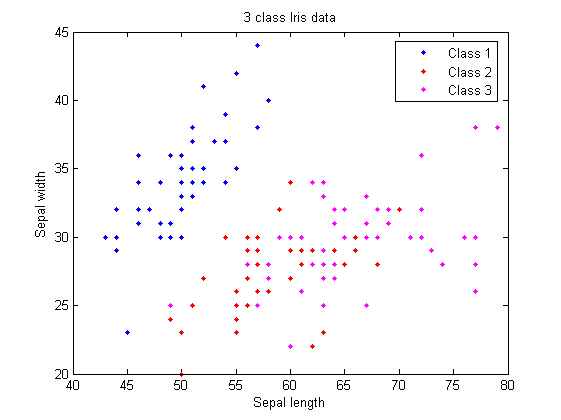
\includegraphics[width=\linewidth]{../Code/FisherIris/svdd/iris_1}
\caption{Scatter plot w.r.t Sepal width and length} 
\end{subfigure}%
\begin{subfigure}{.5\textwidth}
  \centering
  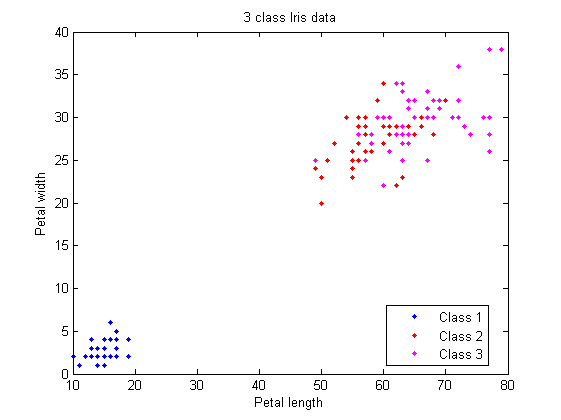
\includegraphics[width=\linewidth]{../Code/FisherIris/svdd/iris_2}
\caption{Scatter plot w.r.t Petal width and length}  
\end{subfigure}
\caption{Scatter plot of the Fisher Iris dataset}
\end{figure}

For the task of Novelty detection , we performed 3 sets of experiments considering each of the three classes as the target class and the rest of the points as outliers. For the purpose of discussion, let's choose class 1 as the target class. We choose 25 points of class 1 to train, and divide the rest into validation and test sets. The parameters $C$ and $\sigma$ were found by performing 10-fold cross validation, and the values of TAER are the average values obtained over 10 random samples of training data. The best values of $C$ and $\sigma$ obtained were $C = 0.4$ and $\sigma = 22.3$. These values were obtained by performing cross validation for the C-SVDD algorithm. For maintaining fairness of results, the same values of $C$ and $\sigma$ were used for the F-SVDD algorithms also.

\subsection{Overlapping classes dataset :} This is the same dataset that was used in our assignments. We use this for visualization and interpreting since it is 2 dimensional. In this dataset, we have 4 classes which are overlapping. The scatter plot of the dataset is shown below :

\begin{figure}
  \centering
  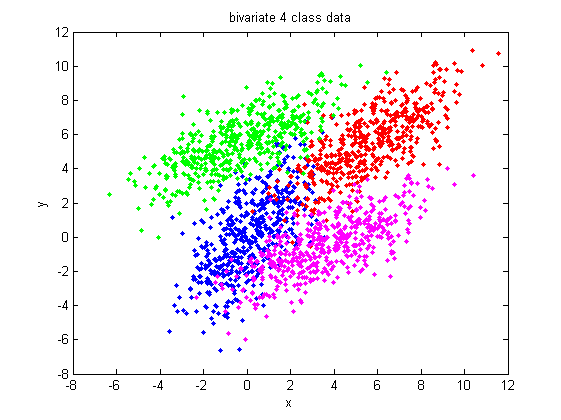
\includegraphics[width=\linewidth]{../Code/overlapping/svdd/data}
\end{figure}


\subsection{Wine recognition Dataset :}\footnote{https://archive.ics.uci.edu/ml/datasets/Wine}  - This is a 13 dimensional dataset of chemical constituents, whose classes are not linearly separable. 


%% \subsection{Double-blind reviewing}

%% This year we are doing double-blind reviewing: the reviewers will not know 
%% who the authors of the paper are. For submission, the NIPS style file will 
%% automatically anonymize the author list at the beginning of the paper.

%% Please write your paper in such a way to preserve anonymity. Refer to
%% previous work by the author(s) in the third person, rather than first
%% person. Do not provide Web links to supporting material at an identifiable
%% web site.

%%\subsection{Electronic submission}
%%
%% \textbf{THE SUBMISSION DEADLINE IS MAY 31st, 2013. SUBMISSIONS MUST BE LOGGED BY
%% 23:00, MAY 31st, 2013, UNIVERSAL TIME}

%% You must enter your submission in the electronic submission form available at
%% the NIPS website listed above. You will be asked to enter paper title, name of
%% all authors, keyword(s), and data about the contact
%% author (name, full address, telephone, fax, and email). You will need to
%% upload an electronic (postscript or pdf) version of your paper.

%% You can upload more than one version of your paper, until the
%% submission deadline. We strongly recommended uploading your paper in
%% advance of the deadline, so you can avoid last-minute server congestion.
%%
%% Note that your submission is only valid if you get an e-mail
%% confirmation from the server. If you do not get such an e-mail, please
%% try uploading again. 


%% \subsection{Keywords for paper submission}
%% Your NIPS paper can be submitted with any of the following keywords (more than one keyword is possible for each paper):

%% \begin{verbatim}
%% Bioinformatics
%% Biological Vision
%% Brain Imaging and Brain Computer Interfacing
%% Clustering
%% Cognitive Science
%% Control and Reinforcement Learning
%% Dimensionality Reduction and Manifolds
%% Feature Selection
%% Gaussian Processes
%% Graphical Models
%% Hardware Technologies
%% Kernels
%% Learning Theory
%% Machine Vision
%% Margins and Boosting
%% Neural Networks
%% Neuroscience
%% Other Algorithms and Architectures
%% Other Applications
%% Semi-supervised Learning
%% Speech and Signal Processing
%% Text and Language Applications

%% \end{verbatim}




%\begin{table}[t]
%\caption{Sample table title}
%\label{sample-table}
%\begin{center}
%\begin{tabular}{ll}
%\multicolumn{1}{c}{\bf PART}  &\multicolumn{1}{c}{\bf DESCRIPTION}
%\\ \hline \\
%Dendrite         &Input terminal \\
%Axon             &Output terminal \\
%Soma             &Cell body (contains cell nucleus) \\
%\end{tabular}
%\end{center}
%\end{table}





\subsubsection*{References}

\small{
[1] Tax, David MJ, and Robert PW Duin. "Support vector data description." Machine learning 54.1 (2004): 45-66. 

[2] Liu, Yi-Hung, Yan-Chen Liu, and Yen-Jen Chen. "Fast support vector data descriptions for novelty detection." Neural Networks, IEEE Transactions on 21.8 (2010): 1296-1313.

[3] Hornik, Kurt, Maxwell Stinchcombe, and Halbert White. "Multilayer feedforward networks are universal approximators." Neural networks 2.5 (1989): 359-366.
}

\end{document}